\chapter{High Intensity Studies}
\label{sec:ch6}

\section{Global RDTs and Intensity-Dependent Effects}

For this chapter, the focus goes back to the Fermilab Recycler Ring. All the experiments and measurements done in Ch. \ref{sec:ch4} were done at low intensities, i.e., less than 1e10 particles per bunch (ppb). Nevertheless, current operations and future operations under PIP-II objectives are done at higher intensities, i.e., 5e10 ppb for current operations and 8e10 ppb for PIP-II. Therefore, it is relevant to explore resonance compensation at higher intensities. 

\section{Space Charge Tune Shift}

The first relevant parameter for high-intensity operation is the space charge tune shift. As mentioned in Ch. \ref{sec:ch2}, the space charge tune shift is an incoherent quantity meaning every particle will feel a different magnitude of this effect. Nevertheless, as shown in Figs. \ref{fig:rrtdmid} and \ref{fig:rrtdhigh}, this incoherent quantity will be contained within a necktie distribution. This necktie profile will define the space charge tune spread. 

A simplification of this equation is:
\begin{equation}
    \label{eq:tunesc}
    \Delta Q_{sc}=\frac{-3 N_b r_0 R S}{4 \sigma_z \beta_L \gamma_L ^2 \varepsilon_{N,95\%}},    
\end{equation}
where $N_b$ is the number of protons per bunch, $r_0=1.535\times 10^{-18}$ meters is the classical radius of the proton, $\sigma_z = 0.5726$ meters is the bunch length, $R = C/(2 \pi)$ is the radius of the Recycler Ring with a circumference of $C=3319.4$ meters, $S=1.596$ is a geometrical factor calculated, $\varepsilon_{N,95\%}$ is the 95\% normalized emittance, and $(\beta_L,\gamma_L)$ are the longitudinal relativistic factors.   

\section{Measurement of Tune Spread}

% \newpage
% \begin{figure}[H]
%     \centering
%     \includegraphics[height=\textheight,keepaspectratio]{chapter6/scts_measure.png}
%     \caption{Tune spread.}
%     \label{fig:dynamictunespread}
% \end{figure}
% \newpage

\begin{figure}[H]
    \centering
    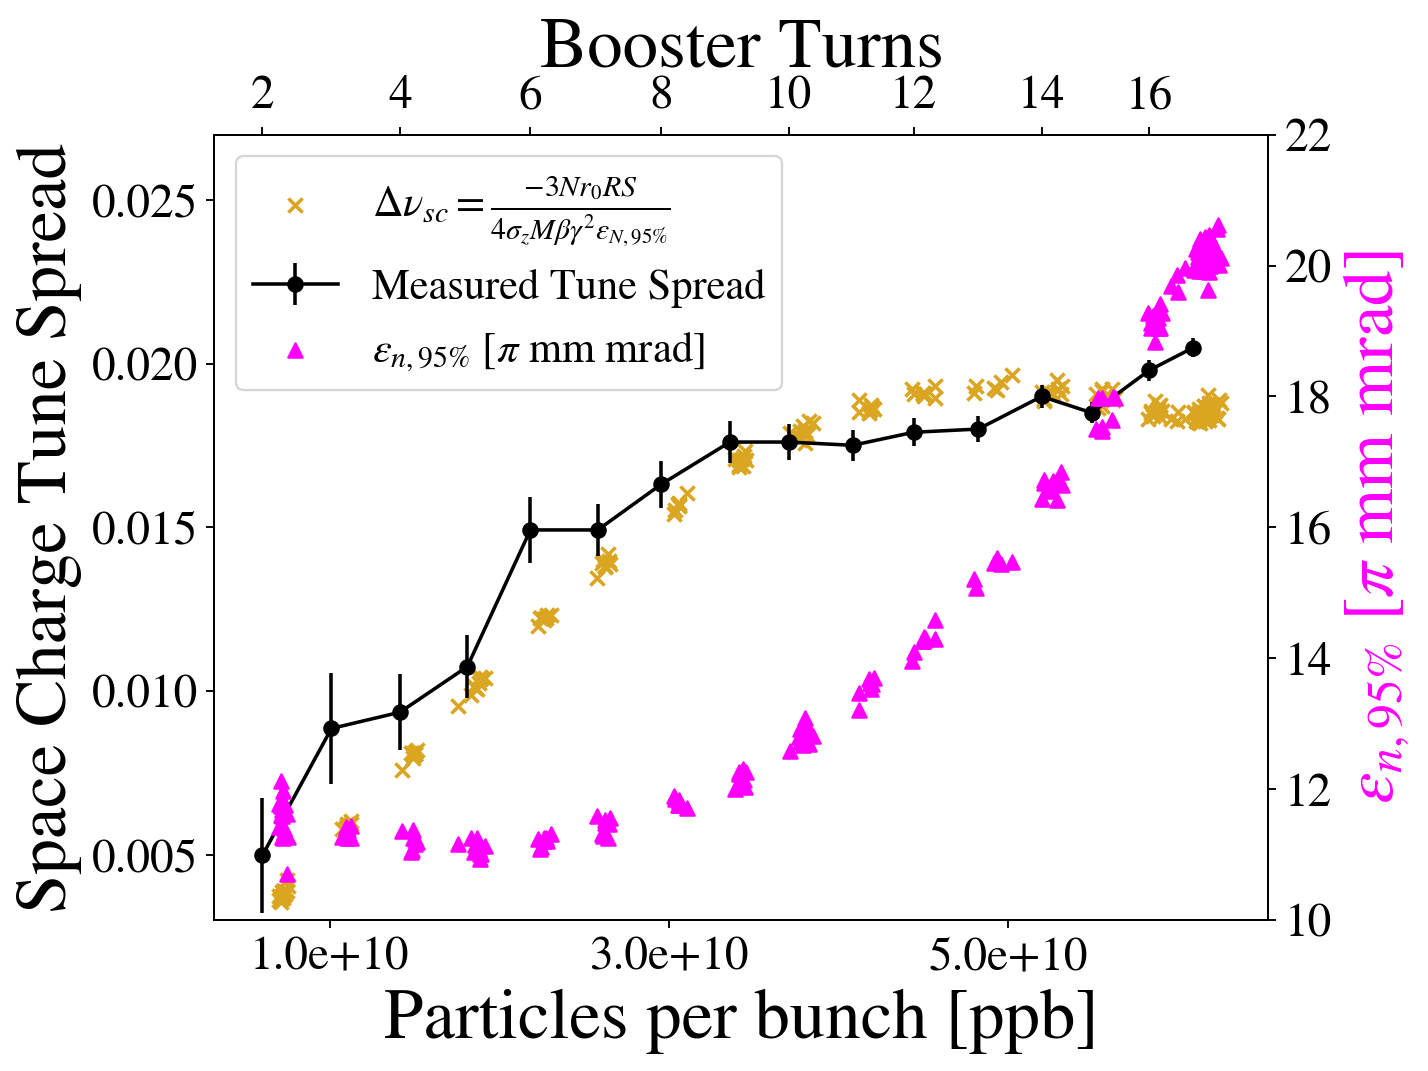
\includegraphics[width=\columnwidth]{chapter6/tune_spread.png}
    \caption{Measurement of tune spread.}
    \label{fig:tunespread}
\end{figure}

\section{Static Tune Scans at Different Intensities}

\begin{figure}[H]
    \centering
    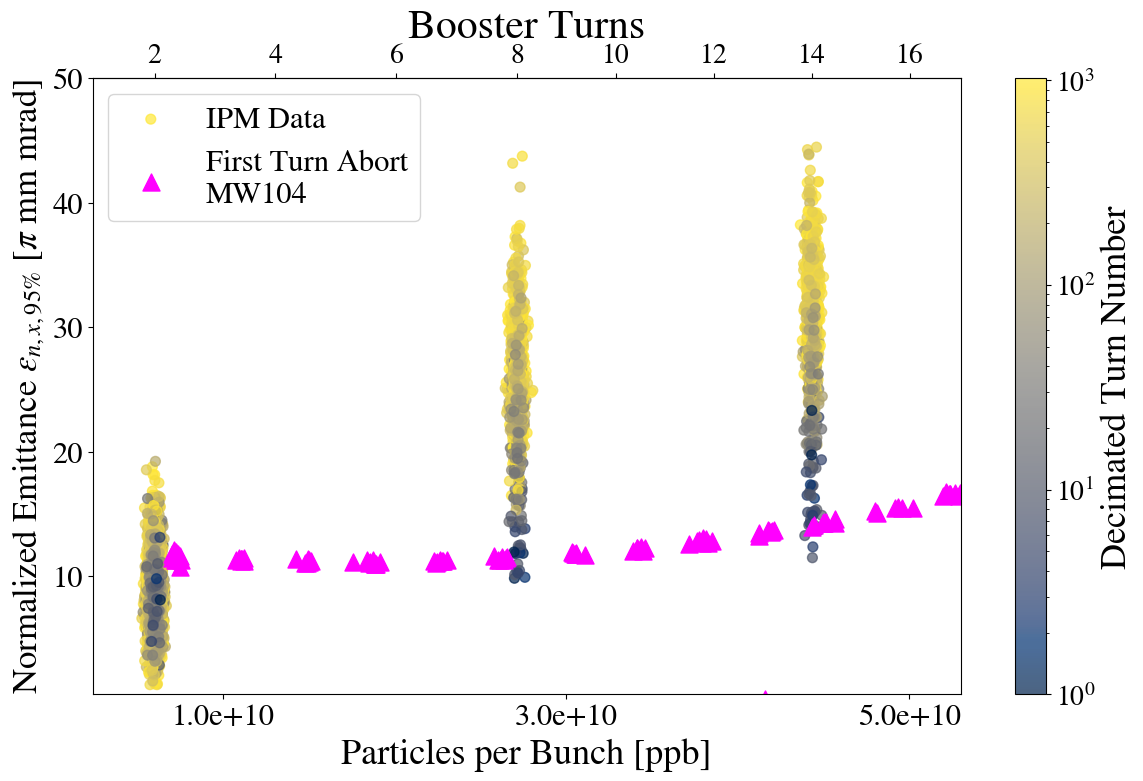
\includegraphics[width=\columnwidth]{chapter6/25370_scatter.png}
    \caption{IPM data and multi-wire first turn abort data for $Q_x=25.370$ at different intensities.}
    \label{fig:25370_scatter}
\end{figure}


\section{Effect of Transverse Dampers}

\begin{figure}[H]
    \centering
    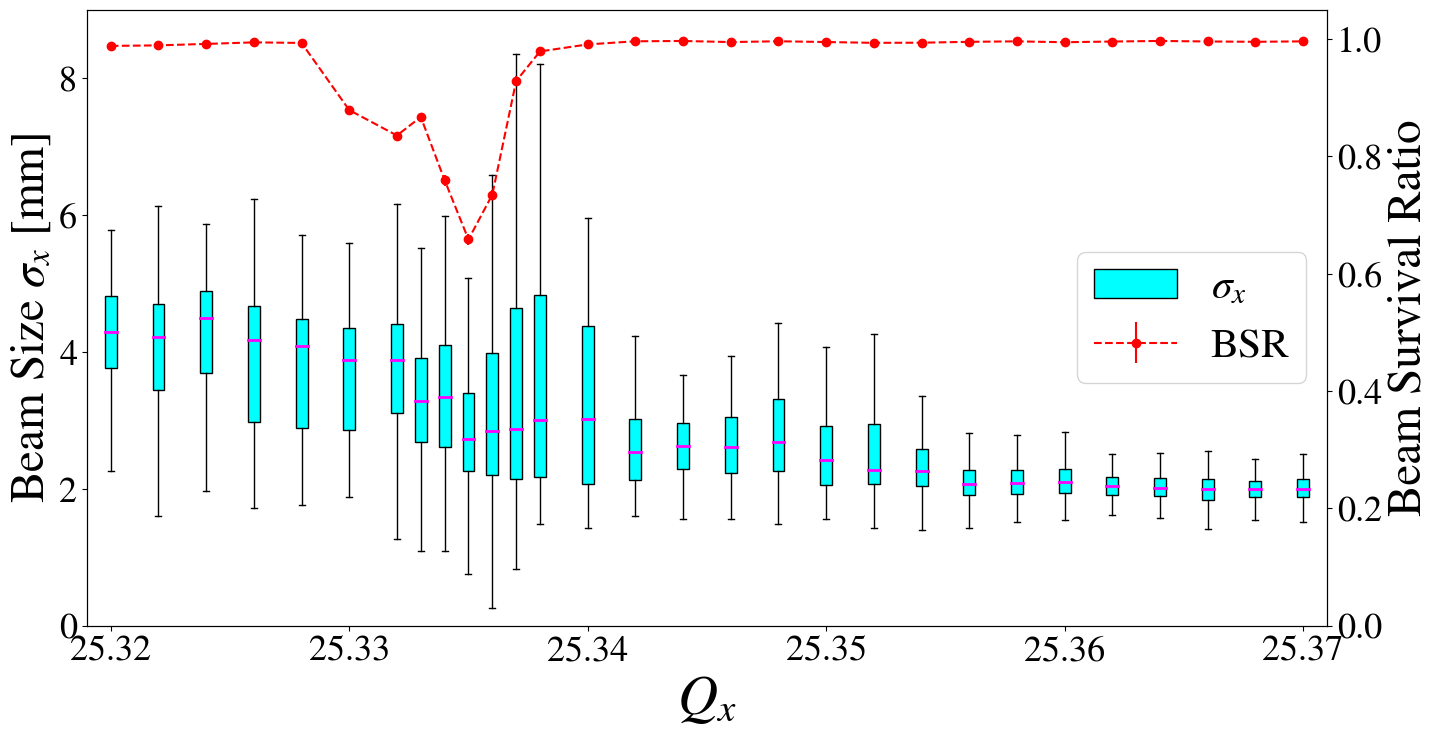
\includegraphics[width=\columnwidth]{chapter6/static2turns_ipm_dampersON.png}
    \caption{Static tune scan with beam survival ratio and IPM data box plots with $3Q_x$ compensation, transverse dampers ON and 2 Booster Turns of equivalent intensity.}
    \label{fig:static2_dampersON}
\end{figure}

\begin{figure}[H]
    \centering
    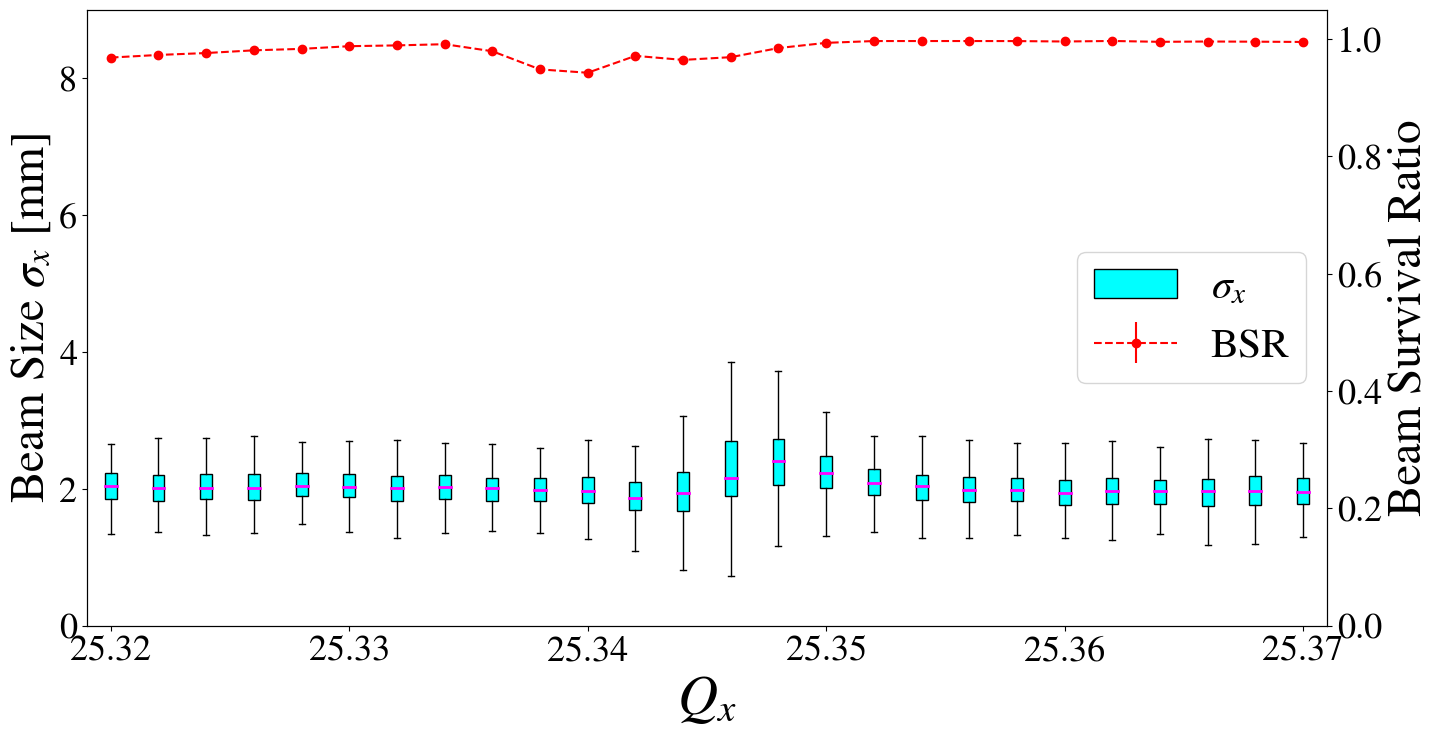
\includegraphics[width=\columnwidth]{chapter6/static2turns_ipm_dampersOFF.png}
    \caption{Static tune scan with beam survival ratio and IPM data box plots with $3Q_x$ compensation, transverse dampers OFF and 2 Booster Turns of equivalent intensity.}
    \label{fig:static2_dampersOFF}
\end{figure}

